\documentclass[{../../master}]{subfiles}
\graphicspath{{../..}}  % 個別コンパイル時の画像パスを解決する

\begin{document}

\section{対向2輪ロボットの実機用URDFモデリング}

早速\textsf{xacro}を用いて実際に対向2輪ロボットの実機用URDFモデリングを行います.
\textsf{xacro}を用いるため,URDFを直接記述することはありませんが,URDFの記述に関する基礎知識が必要になります.
このセクションではURDF記述のチュートリアルについては取り扱わず,より実践的な内容を説明します.
URDFモデリングのチュートリアルはWeb上に大量に存在します.
この小節を読む前に,そちらを参照して基礎知識を身に付けてください.

これからモデリングする対向2輪ロボットのスケッチを図\ref{fig:mobile_robot_structure}に,リンクとジョイントのグラフを図に示します.

\begin{figure}[ht]
  \centering
  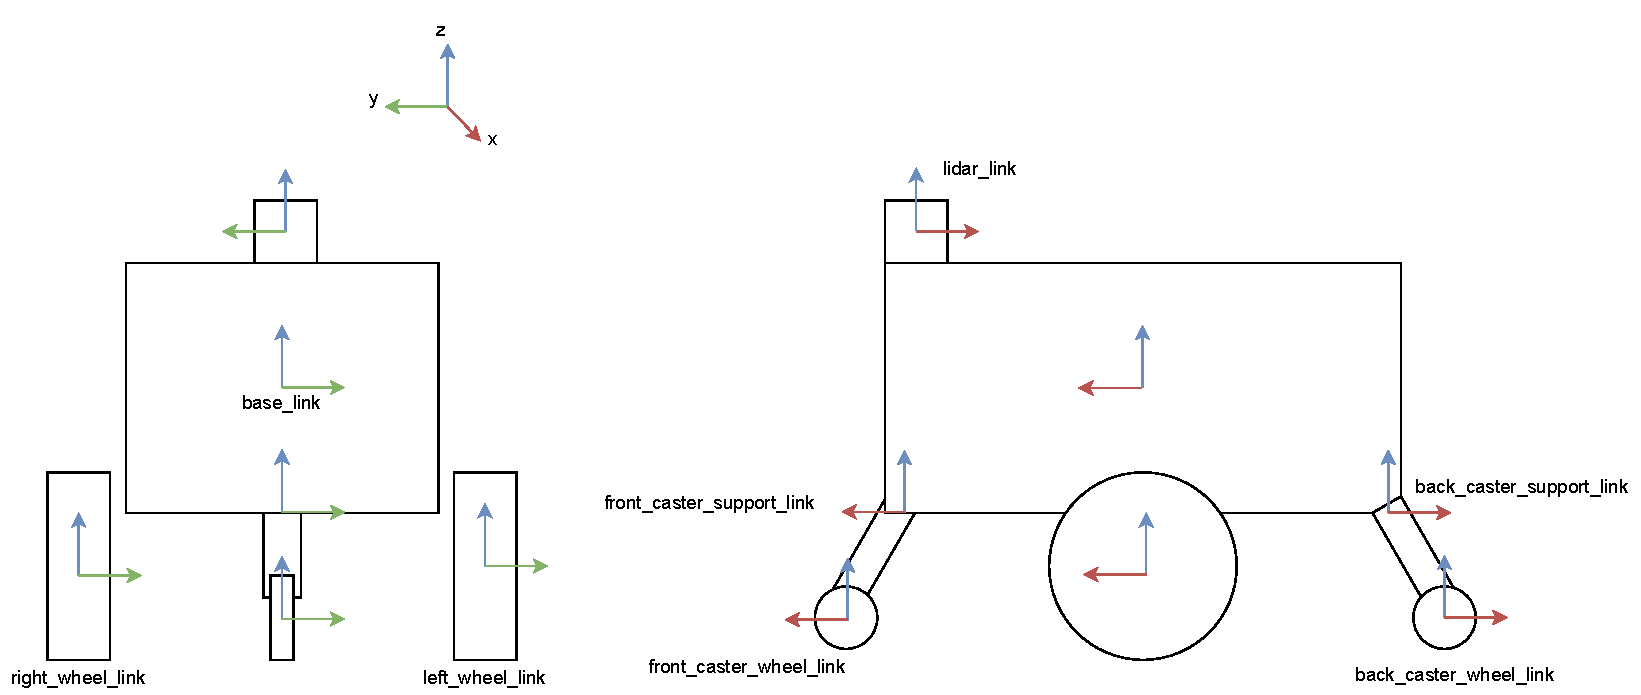
\includegraphics[width=100truemm, clip]{images/mobile_robot_structure.drawio.pdf}
  \caption{Link Structure of Diff-Drive Mobile Robot}
  \label{fig:mobile_robot_structure}
\end{figure}

トップレベルのリンクとして\textsf{base\_footprint}(空のリンク)があり,その下に\textsf{base\_link}があります.
ホイール,センサ,キャスターのリンクはすべて\textsf{base\_link}の子リンクです.

\end{document}